\documentclass[border=10pt]{standalone}
\usepackage[svgnames]{xcolor}
\usepackage{amsmath}
\usepackage{pgfplots}
\pgfplotsset{compat=newest}
\usepackage[sfdefault]{FiraSans}
\usepackage{FiraMono}
\renewcommand*\familydefault{\sfdefault}
\begin{document}
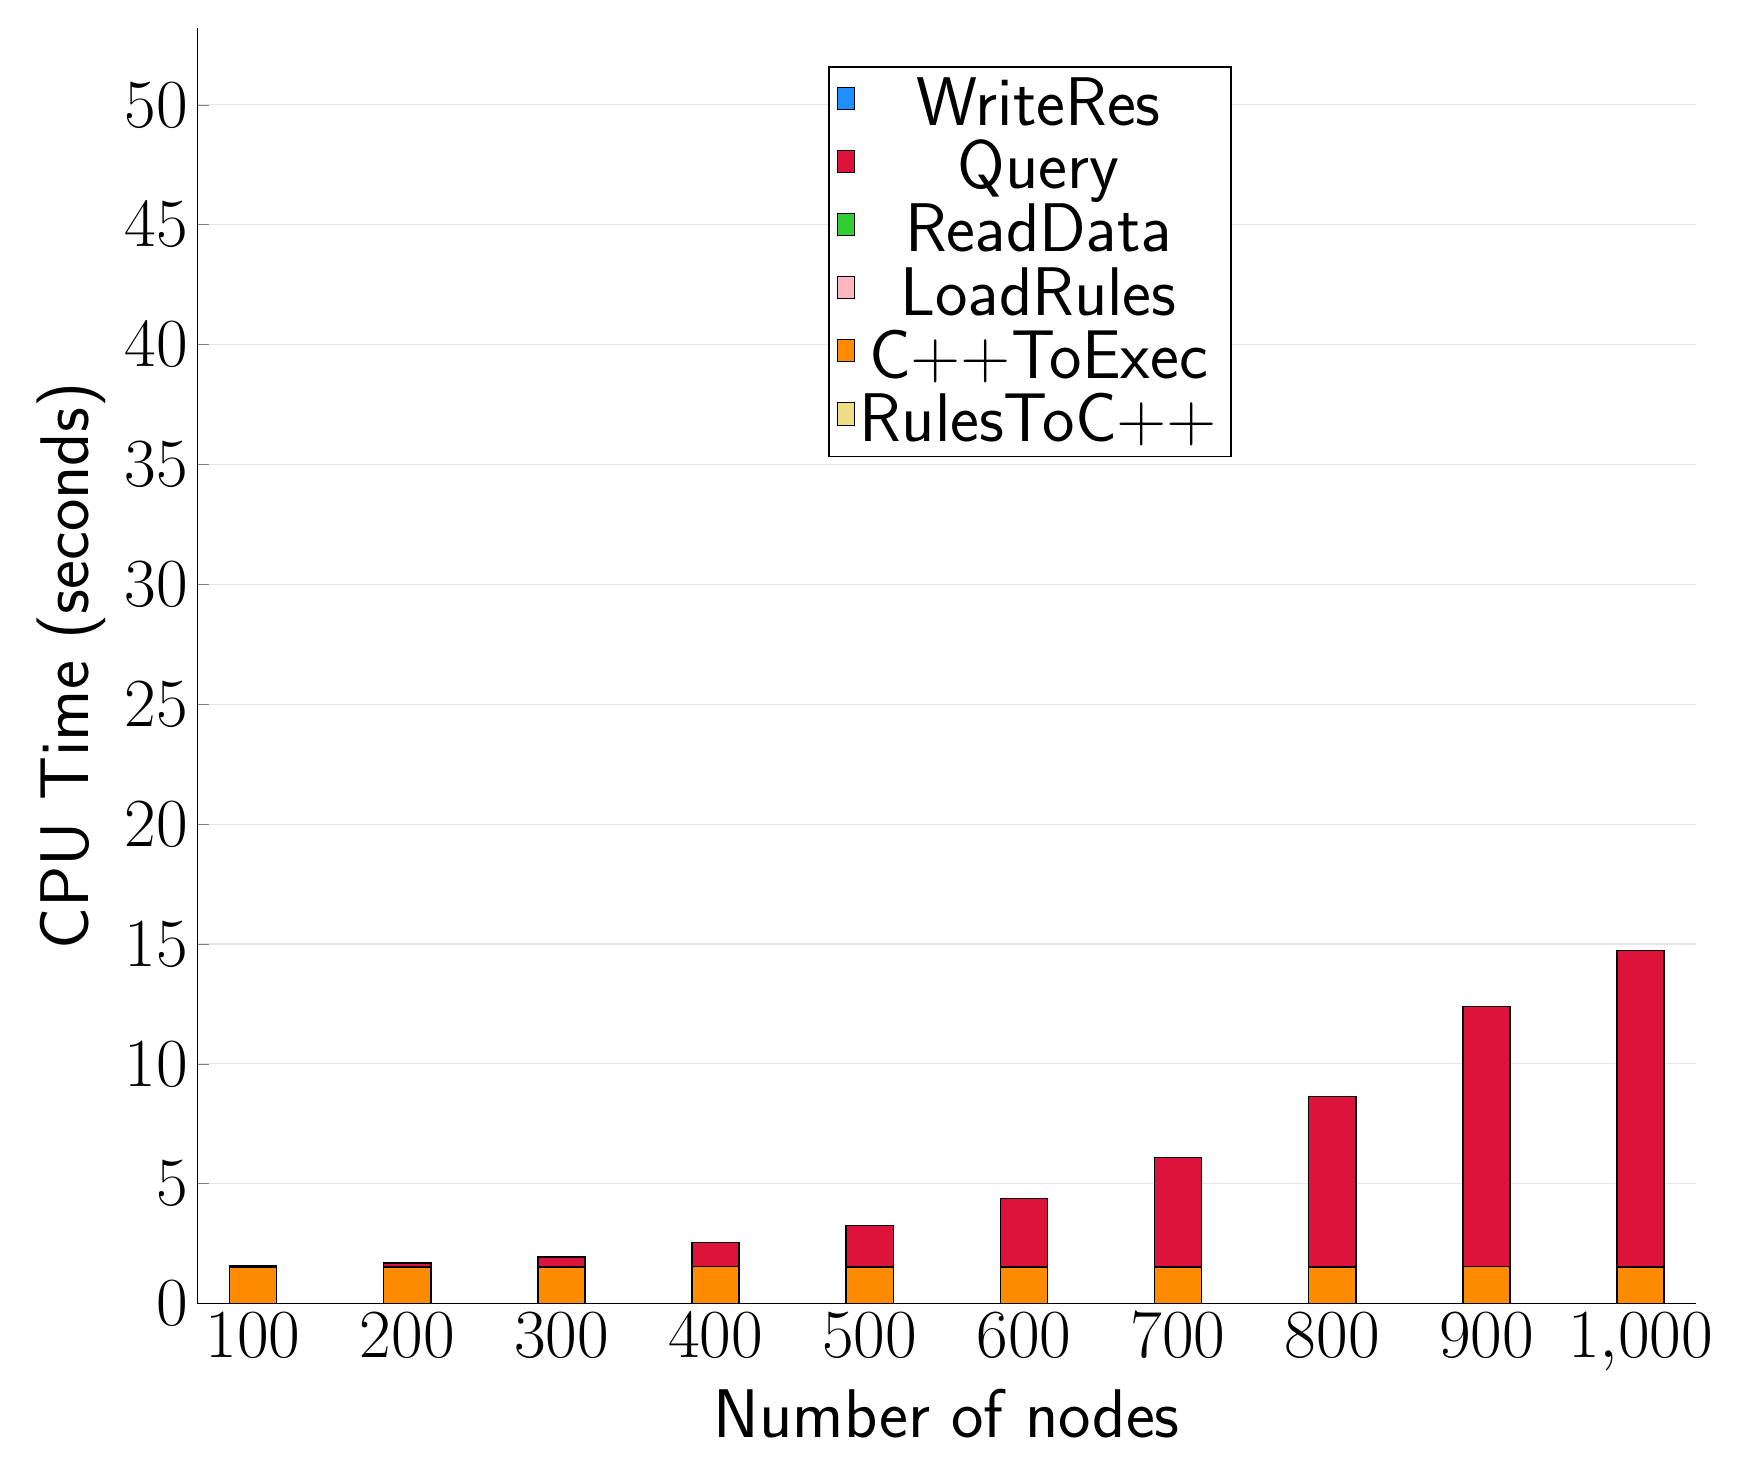
\begin{tikzpicture}
\begin{axis}[
   ybar stacked,
   width=1.7\textwidth,
   bar width=0.6cm,
   ymajorgrids, tick align=inside,
   major grid style={draw=gray!20},
   xtick=data,
   ymin=0, ymax=53.1968,
   axis x line*=bottom,
   axis y line*=left,
   enlarge x limits=0.04,
   legend style={
       at={(0.69, 0.97)},
       anchor=north east,
       legend columns=1,
       font=\Huge,
   },
   ylabel={CPU Time (seconds)},
   xlabel={Number of nodes},
   label style={font=\Huge},
   tick label style={font=\Huge},
]
\addlegendimage{fill=DodgerBlue, draw=black, line width=0.2pt}
\addlegendentry{WriteRes}
\addlegendimage{fill=Crimson, draw=black, line width=0.2pt}
\addlegendentry{Query}
\addlegendimage{fill=LimeGreen, draw=black, line width=0.2pt}
\addlegendentry{ReadData}
\addlegendimage{fill=LightPink, draw=black, line width=0.2pt}
\addlegendentry{LoadRules}
\addlegendimage{fill=DarkOrange, draw=black, line width=0.2pt}
\addlegendentry{C++ToExec}
\addlegendimage{fill=LightGoldenrod, draw=black, line width=0.2pt}
\addlegendentry{RulesToC++}
\addplot +[fill=LightGoldenrod, draw=black, line width=0.55pt] coordinates {
(100, 0.004000000000000001)
(200, 0.008000000000000002)
(300, 0.006000000000000001)
(400, 0.006000000000000001)
(500, 0.008000000000000002)
(600, 0.006000000000000001)
(700, 0.010000000000000002)
(800, 0.008000000000000002)
(900, 0.004000000000000001)
(1000, 0.004000000000000001)
};
\addplot +[fill=DarkOrange, draw=black, line width=0.55pt] coordinates {
(100, 1.5300000000000002)
(200, 1.5299999999999998)
(300, 1.532)
(400, 1.5340000000000003)
(500, 1.5239999999999998)
(600, 1.528)
(700, 1.516)
(800, 1.522)
(900, 1.548)
(1000, 1.52)
};
\addplot +[fill=LightPink, draw=black, line width=0.55pt] coordinates {
(100, 0.0001648)
(200, 0.0001528)
(300, 0.00015439999999999999)
(400, 0.0001618)
(500, 0.000149)
(600, 0.00015900000000000002)
(700, 0.00015580000000000002)
(800, 0.0001702)
(900, 6.48e-05)
(1000, 2.98e-05)
};
\addplot +[fill=LimeGreen, draw=black, line width=0.55pt] coordinates {
(100, 0.0011976)
(200, 0.0019018)
(300, 0.002254)
(400, 0.0032624)
(500, 0.0031646)
(600, 0.003929)
(700, 0.0053058)
(800, 0.005422000000000001)
(900, 0.004007600000000001)
(1000, 0.0031514)
};
\addplot +[fill=Crimson, draw=black, line width=0.55pt] coordinates {
(100, 0.0366682)
(200, 0.1465454)
(300, 0.4091076)
(400, 1.0139019999999999)
(500, 1.7210180000000002)
(600, 2.8472560000000002)
(700, 4.554384)
(800, 7.103302000000001)
(900, 10.837399999999999)
(1000, 13.196800000000001)
};
\addplot +[fill=DodgerBlue, draw=black, line width=0.55pt] coordinates {
(100, 0.00026220000000000003)
(200, 0.0002886)
(300, 0.0003336)
(400, 0.000334)
(500, 0.0004006)
(600, 0.0003690000000000001)
(700, 0.00043620000000000003)
(800, 0.00047819999999999997)
(900, 0.00045240000000000005)
(1000, 0.0005186)
};
\end{axis}
\end{tikzpicture}

\end{document}
